    \section{Obliczenia Teoretyczne}
    \label{sec:calculations}
Do zaprojektowania filtru pasmowoprzepustowego o częstotliwościach 
granicznych 1 Hz i 300 Hz wykorzystaliśmy wzory z książki ``Op Amps for 
Everyone''\cite{SLOA088}. Zawarte są w niej wskazówki do projektowania 
flitrów, jak i obliczenia dla poszczególnych topoligii. \\

Wybrany filtr aktywny jest filtrem pasmowoprzepustowym 3 rzędu. Można 
w jego strukturze zauważyć trzy podstawowe konfiguracje - filtr 
dolnoprzepustowy aktywny (\ref{eq:lpf}), Sallen-Key (\ref{eq:sk}) 
dla spełnionego warunku (\ref{eq:sk_cond}) 
oraz filtr górnoprzepustowy pasywny (\ref{eq:hpf}). 
Na podstawie parametrów dla filtru Butterwortha 3 rzędu: 
\begin{table}[H]
\centering
\renewcommand{\arraystretch}{1.2}
\begin{tabular}{|l|c|c|}
\hline
\textbf{} & \textbf{i = 1} & \textbf{i = 2} \\
\hline
a & 0,7560 & 0,9996 \\
\hline
b & 0 & 0,4772 \\
\hline
k & 1,323 & 1,414 \\
\hline
Q & - & 0,69 \\
\hline
\end{tabular}
\end{table}
oraz wzorów z wspomnianej powyżej książki, obliczyliśmy wartości
elementów dla poszczególnych sekcji filtru przyjmując wartość pojemności
$C_1 = C_2 = 100 nF$.

\begin{equation}
\label{eq:lpf}
R_{1} = 
\frac{a_1}{2 \pi f_c C_1}
 = 
\frac{0,7560}{2 \pi \cdot 300Hz \cdot 100nF}
 = 
4,01 k\Omega
\end{equation}

\begin{equation}
\label{eq:sk_cond}
C_3 \geq 
C_2 \cdot \frac{4b_2}{a_2^2}
 = 
100nF \cdot \frac{4 \cdot 0,4772}{0,9996^2}
 = 
100 nF \cdot 1,91033
 = 
191,033 nF \approx 200 nF
\end{equation}

\begin{equation}
\label{eq:sk}
\begin{aligned}
R_{2,3} &= 
\frac{a_2 C_3 \pm \sqrt{a_2^2 C_3^2 - 4b_2 C_2 C_3}}{4 \pi f_c C_2 C_3}
 = \\ &= 
\frac{0,9996 \cdot 200nF \pm \sqrt{0,9996^2 \cdot (200nF)^2 - 
4 \cdot 0,4772 \cdot 100nF \cdot 200nF}}
{4 \pi \cdot 300Hz \cdot 100nF \cdot 200nF} \\
R_2 &\approx 2,09 k\Omega \\
R_3 &\approx 3,212 k\Omega
\end{aligned}
\end{equation}

\begin{equation}
\label{eq:hpf}
R_{4} = \frac{1}{2 \pi f_c C_4} 
 = 
\frac{1}{2 \pi \cdot 1Hz \cdot 470nF}
 = 
338,6 k\Omega
\end{equation}

% --- photo: freq response filtra nr 1 ---
\begin{figure}[H]
\centering
\setlength{\fboxrule}{2pt}
\setlength{\fboxsep}{0pt}
\fbox{
    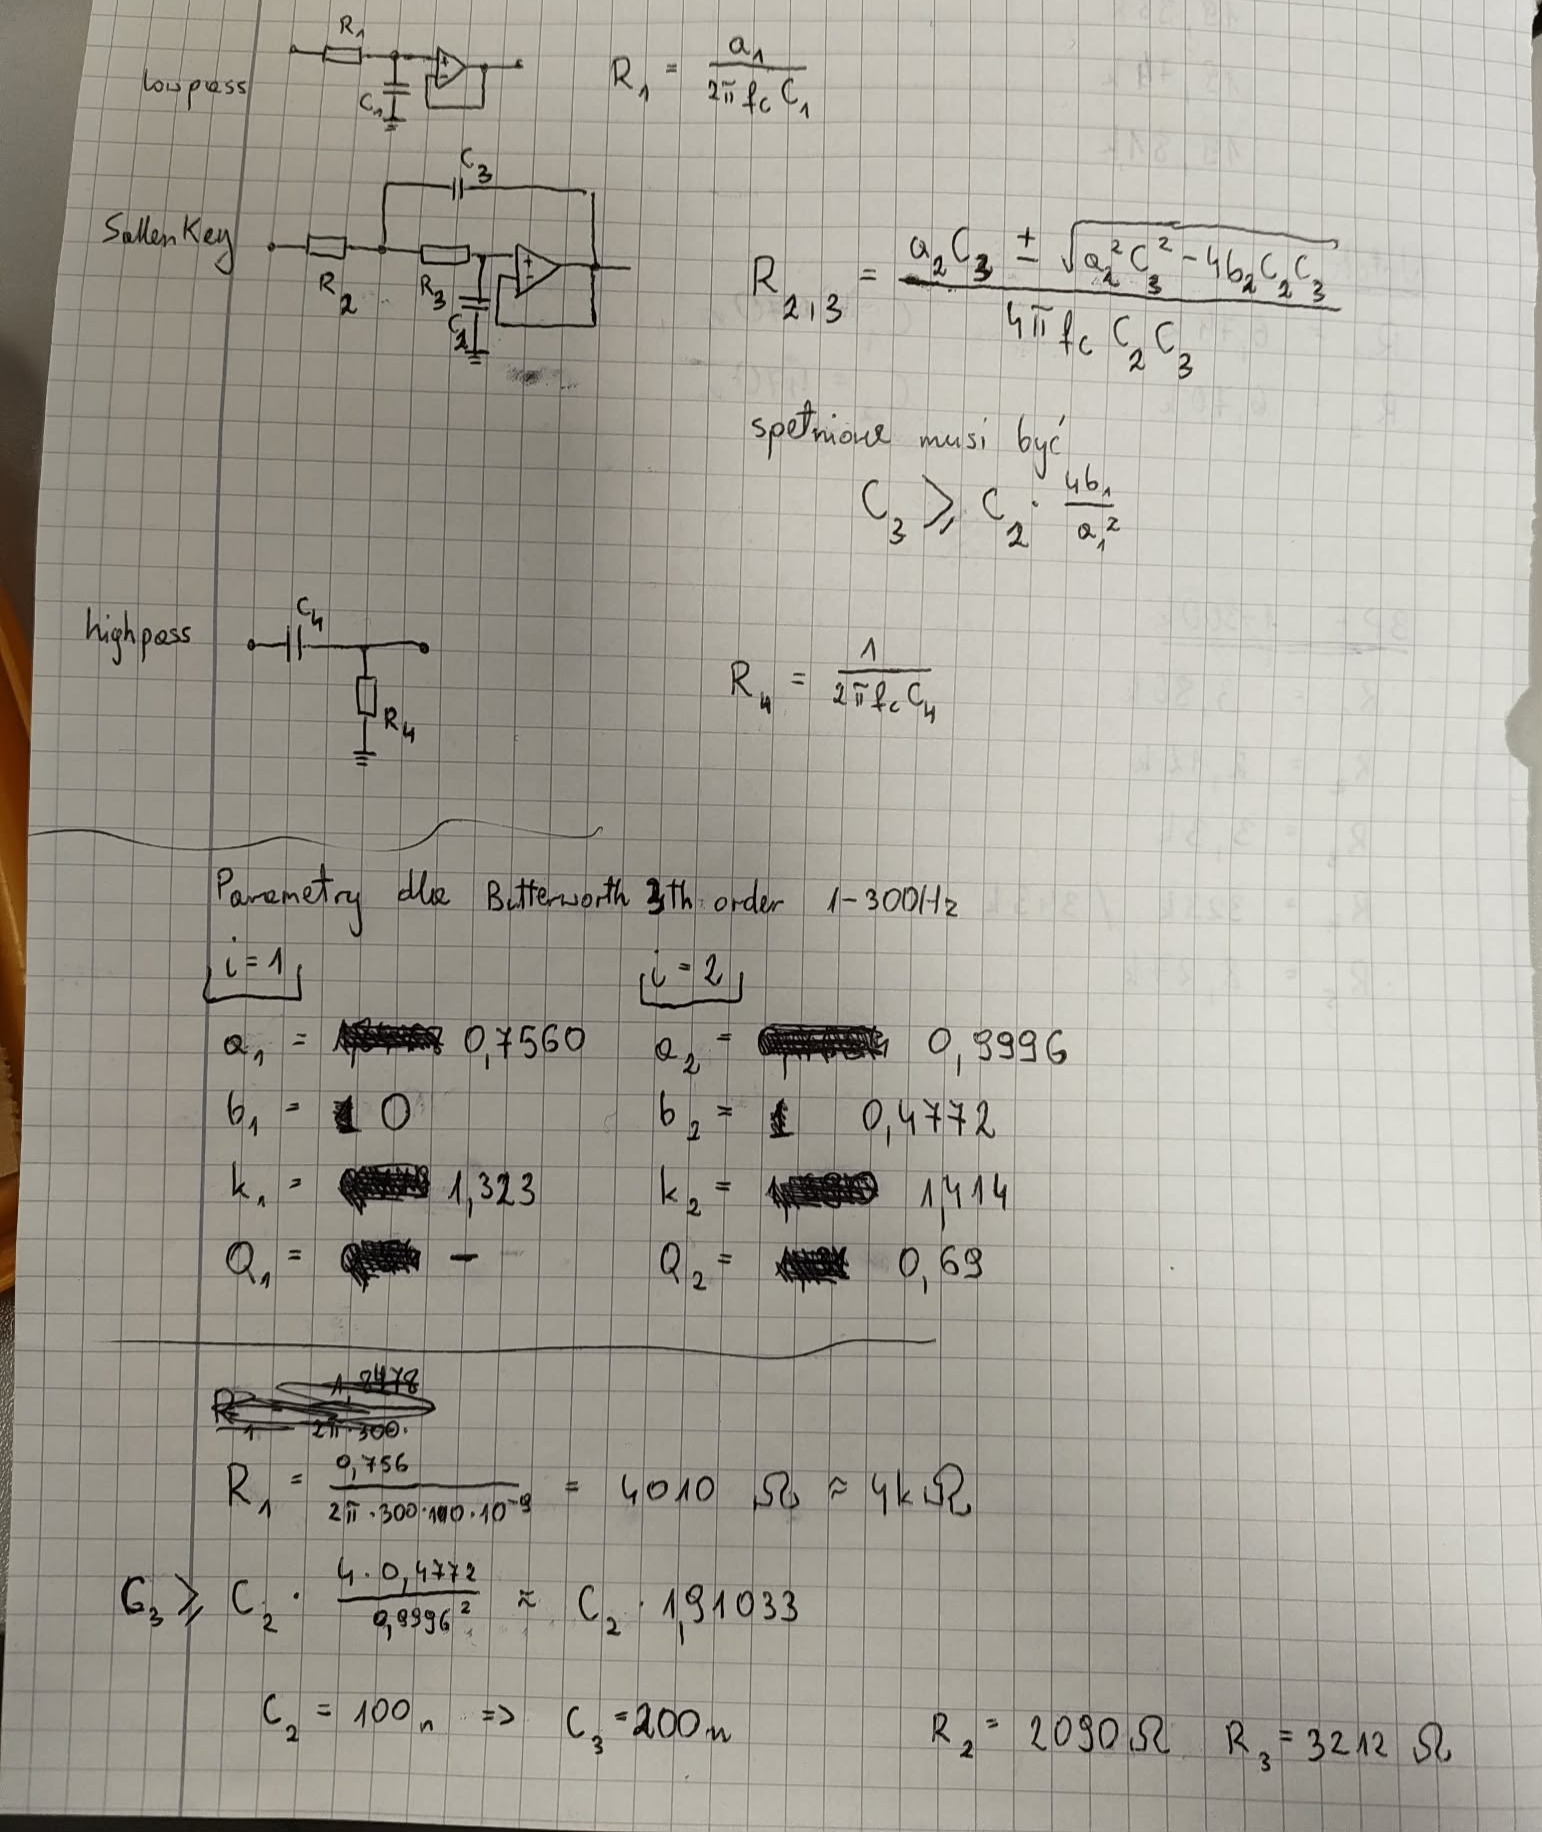
\includegraphics[width=0.8\textwidth]{figures/calculations_official_paper.jpg}
}
\caption{Dowód że liczyliśmy \dWinkey[1.5].}
\end{figure}
% --- end photo ---

